\documentclass[10pt]{article}
\usepackage[verbose, a4paper, hmargin=2.5cm, vmargin=2.5cm]{geometry}

\usepackage{fontspec}
\usepackage{ctex}
\usepackage{paratype}

\usepackage{amsmath}
\usepackage{amssymb}
\usepackage{amsfonts}
\usepackage{esint}
\usepackage{stmaryrd}

\usepackage[mathbf=sym]{unicode-math}
\setmainfont{STIX Two Text}
\setmathfont{STIX Two Math}

\setsansfont{Arial}
\setmonofont{Courier New}

\usepackage{makecell}
\usepackage{wasysym}
\usepackage{pifont}
\usepackage[export]{adjustbox}
\usepackage{graphicx}
\usepackage{mdframed}
\usepackage{booktabs,array,multirow}
\usepackage{tabularx}
\usepackage{hyperref}
\hypersetup{colorlinks=true, linkcolor=blue, filecolor=magenta, urlcolor=cyan,}
\urlstyle{same}
\usepackage[most]{tcolorbox}
\usepackage{tikz}
\usepackage{needspace}  % 防止跨页

% 定义留白命令 - 用于教师板书
\newcommand{\boardspace}[1]{%
  \par\vspace{#1}
}

% 定义中难题留白（大幅留白供教师板书）
\newcommand{\hardboardspace}{%
  \par\vspace{5cm}
  \hfill\textit{（此处留白供课堂讲解）}
  \par\vspace{1cm}
}

% 定义大题留白
\newcommand{\largeboardspace}{%
  \par\vspace{8cm}
  \hfill\textit{（此处留白供课堂讲解与板书推导）}
  \par\vspace{1cm}
}

% 题目不跨页环境
\newenvironment{questionblock}[1]{%
  \needspace{3\baselineskip}%
  \noindent\textbf{#1.}%
}{%
  \par\vspace{1em}%
}

\definecolor{mygray}{RGB}{240,240,240}
\tcbset{
  colback=mygray,
  boxrule=0pt,
}
\graphicspath{ {./images/} }
\newcommand{\HRule}{\begin{center}\rule{0.9\linewidth}{0.2mm}\end{center}}
\newcommand{\customfootnote}[1]{
  \let\thefootnote\relax\footnotetext{#1}
}
\newcommand{\lt}{\mathrel{<}}
\newcommand{\gt}{\mathrel{>}}
\newcommand*\circled[1]{\tikz[baseline=(char.base)]{\node[shape=circle,draw,inner sep=1.5pt] (char) {\small #1};}}
\setcounter{MaxMatrixCols}{256}

\begin{document}

\begin{center}
\Large\textbf{2026届嘉定区高三下二模数学试卷}\\[0.5em]
\normalsize\textit{（学生版·课堂使用）}
\end{center}

\section*{一、填空题（第1-9题每题4分，第10-12题每题5分，共51分）}

\begin{questionblock}{1}
已知集合 \(A = \left\{  {a,{a}^{2}}\right\}\) ，且 \(1 \in  A\) ，则 \(a =\) ___.
\end{questionblock}

\boardspace{1.5cm}

\begin{questionblock}{2}
解不等式 \(\frac{1}{x} > 1\) ,则不等式的解集是___
\end{questionblock}

\boardspace{1.5cm}

\begin{questionblock}{3}
已知角 \(\alpha\) 的终边经过点 \(P\left( {1, - 2}\right)\) ，则 \(\sin \alpha  =\) ___.
\end{questionblock}

\boardspace{1.5cm}

\begin{questionblock}{4}
已知 \(\left\{  {a}_{n}\right\}\) 是等差数列， \({a}_{6} = 1,{a}_{26} = {11}\) ，则 \({a}_{2026} =\) ___.
\end{questionblock}

\boardspace{1.5cm}

\begin{questionblock}{5}
双曲线 \(\frac{{x}^{2}}{9} - \frac{{y}^{2}}{16} = 1\) 的渐近线方程是___.
\end{questionblock}

\boardspace{1.5cm}

\begin{questionblock}{6}
由0,1,2,3,4组成没有重复数字的三位数的个数是___
\end{questionblock}

\boardspace{1.5cm}

\begin{questionblock}{7}
函数 \(y = {\sin }^{4}x + {\cos }^{4}x\) 的最小正周期是___.
\end{questionblock}

\boardspace{1.5cm}

\begin{questionblock}{8}
已知函数 \(y = {x}^{3} + {x}^{2} + {ax}\) 有三个不同的零点,则实数 \(a\) 的取值范围是___
\end{questionblock}

\boardspace{1.5cm}

\begin{questionblock}{9}
已知向量 \(\overrightarrow{a} = \left( {\cos x,\sin x}\right) ,\overrightarrow{b} = \left( {3,\sqrt{3}}\right)\) ，且 \(x \in  \left\lbrack  {0,\frac{\pi }{2}}\right\rbrack\) ，则 \(\overrightarrow{a}\) 在 \(\overrightarrow{b}\) 方向上的数量投影的取值范围为 ___
\end{questionblock}

\boardspace{1.5cm}

\begin{questionblock}{10}
已知正四面体上的四个面上分别写有 1、2、3、4，游戏中甲、乙轮流抛掷该四面体，谁抛出底面数字等于 4 则获胜且游戏结束. 甲先开始，则甲获胜的概率为___.
\end{questionblock}

\hardboardspace

\begin{questionblock}{11}
将函数 \(y = {x}^{2}, x \in  \left\lbrack  {0,1}\right\rbrack\) 的图象绕坐标原点逆时针方向旋转角 \(\theta \left( {0 \leq  \theta  \leq  \alpha }\right)\) 得到曲线 \(C\) . 若对于每一个角 \(\theta\) ，曲线 \(C\) 都是一个函数的图象，则 \(\alpha\) 的最大值为___.
\end{questionblock}

\hardboardspace

\begin{questionblock}{12}
在包装设计中,常用长度和宽度描述物体体型. 长度 \(l\left( V\right)\) 定义为物体上最远两点间的距离,宽度 \(t\left( V\right)\) 定义为能夹住物体的两平行平面间的最小距离, 即存在一对平行平面, 使得物体上的所有点均位于两平面之间 (包括平面上). 现有一圆柱,其底面半径 \(R\) 与高 \(h\) 可任意调节,则 \(\frac{l\left( V\right) }{t\left( V\right) }\) 的最小值为___
\end{questionblock}

\hardboardspace

\section*{二、单选题（每题5分，共20分）}

\begin{questionblock}{13}
已知陈述句 \(\alpha\) 是 \(\beta\) 的充分非必要条件. 若集合 \(M = \{ x \mid  x\) 满足 \(\alpha \} , N = \{ x \mid  x\) 满足 \(\beta \}\) ,则 \(M\) 与 \(N\) 的关系为 ( )

A. \(M \subset  N\) B. \(M \supset  N\) C. \(M = N\) D. \(M \cap  N = \varnothing\)
\end{questionblock}

\boardspace{1.5cm}

\begin{questionblock}{14}
生物学家在研究动物体重 \(W\) (单位: \(\mathrm{g}\) ) 与脉搏率 \(f\) (单位: 次 \(\cdot  {\mathrm{{min}}}^{-1}\) ) 的关系时,获得了右表的数据, 令 \(x = \ln W,\;y = \ln f\) ,并拟合线性回归方程 \(\widehat{y} = \widehat{a}x + \widehat{b}\) . 根据已知数据,下列说法正确的是 ( )

<table><tr><td>动物名</td><td>体重 \(W/\mathrm{g}\)</td><td>脉搏率 \(f/\left( {\text{ 次 } \cdot  {\mathrm{{min}}}^{-1}}\right)\)</td></tr><tr><td>鼠</td><td>25</td><td>670</td></tr><tr><td>豚鼠</td><td>300</td><td>300</td></tr><tr><td>兔</td><td>2000</td><td>205</td></tr><tr><td>小狗</td><td>5000</td><td>120</td></tr><tr><td>大狗</td><td>30000</td><td>85</td></tr><tr><td>羊</td><td>50000</td><td>70</td></tr></table>

<table><tr><td>马</td><td>450000</td><td>38</td></tr></table>

A. 变量 \(x\) 与 \(y\) 成正相关,且 \(\widehat{b} > 0\) B. 变量 \(x\) 与 \(y\) 成负相关,且 \(\widehat{b} < 0\)

C. 变量 \(x\) 与 \(y\) 成正相关,且 \(\widehat{b} < 0\) D. 变量 \(x\) 与 \(y\) 成负相关,且 \(\widehat{b} > 0\)
\end{questionblock}

\boardspace{1.5cm}

\begin{questionblock}{15}
设数列 \(\left\{  {a}_{n}\right\}\) 满足 \({a}_{1} = 1\) ,且 \({a}_{n + 1} = \frac{\left( {{\lambda n} - 2}\right)  \cdot  {a}_{n}}{{n}^{2} + 1}\) ,其中 \(\lambda  \in  \mathbf{R}\) . 下列选项中错误的是 ( )

A. 存在 \(\lambda\) ,使得存在正整数 \(\mathbf{N}\) ,当 \(n \geq  \mathbf{N}\) 时,总有 \({a}_{n + 1} < {a}_{n}\)

B. 存在 \(\lambda\) ,使得不存在正整数 \(\mathbf{N}\) ,当 \(n \geq  \mathbf{N}\) 时,总有 \({a}_{n + 1} > {a}_{n}\)

C. 对任意 \(\lambda\) ，都不存在正整数 \(\mathbf{N}\) ，使得当 \(n \geq  \mathbf{N}\) 时，总有 \({a}_{n + 1} > {a}_{n}\)

D. 存在 \(\lambda\) ,使得不存在正整数 \(\mathbf{N}\) ,当 \(n \geq  \mathbf{N}\) 时,总有 \({a}_{n + 1} < {a}_{n}\)
\end{questionblock}

\hardboardspace

\begin{questionblock}{16}
对任意平面向量 \(\overrightarrow{a}\text{ 、 }\overrightarrow{b}\text{ 、 }\overrightarrow{c}\) 及任意实数 \(\lambda\) ,已知运算 \(\odot\) 满足以下三条性质: (I) \(\overrightarrow{a} \odot  \overrightarrow{b} = \overrightarrow{b} \odot  \overrightarrow{a}\) ; (II) \(\left( {\overrightarrow{a} + \overrightarrow{b}}\right)  \odot  \overrightarrow{c} = \overrightarrow{a} \odot  \overrightarrow{c} + \overrightarrow{b} \odot  \overrightarrow{c}\) ; (III) \(\left( {\lambda \overrightarrow{a}}\right)  \odot  \overrightarrow{b} = \lambda \left( {\overrightarrow{a} \odot  \overrightarrow{b}}\right)\) . 则下列选项中一定成立的是 ( )

A. 若 \(\overrightarrow{a} \odot  \overrightarrow{b} = 0\) ,则 \(\overrightarrow{a} = \overrightarrow{0}\) 或 \(\overrightarrow{b} = \overrightarrow{0}\) B. \(\left| {\overrightarrow{a} \odot  \overrightarrow{b}}\right|  = \left| \overrightarrow{a}\right|  \cdot  \left| \overrightarrow{b}\right|\)

C. \(\left( {\overrightarrow{a} - \overrightarrow{b}}\right)  \odot  \left( {\overrightarrow{a} - \overrightarrow{b}}\right)  = \overrightarrow{a} \odot  \overrightarrow{a} - 2\overrightarrow{a} \odot  \overrightarrow{b} + \overrightarrow{b} \odot  \overrightarrow{b}\;\) D. \(\overrightarrow{a} \odot  \overrightarrow{a} \geq\)
\end{questionblock}

\hardboardspace

\section*{三、解答题（共79分）}

\begin{questionblock}{17}
在复平面内,已知点 \(A\text{ 、 }B\text{ 、 }C\) 对应的复数分别为 \({z}_{A} = 0\text{ 、 }{z}_{B} = 6\text{ 、 }{z}_{C} = 4 + 3\mathrm{i}\) ,其中 \(i\) 是虚数单位.

(1)求 \(\cos \angle {ACB}\) 的值；

(2)若复数 \(z\) 满足 \(\left| {z - {z}_{A}}\right|  = \left| {z - {z}_{B}}\right|  = \left| {{z}_{B} - {z}_{C}}\right|\) ，求 \(z\) .
\end{questionblock}

\boardspace{1.5cm}

\newpage

\begin{questionblock}{18}
如图，在 \(\bigtriangleup  {ABC}\) 中， \(\angle {ACB} = {90}^{ \circ  }\) ， \({DA}\bot\) 平面 \({ABC}\) ， \(M\) ， \(N\) 分别是线段 \({AC}\) 、 \({DB}\) 的中点.

\begin{center}
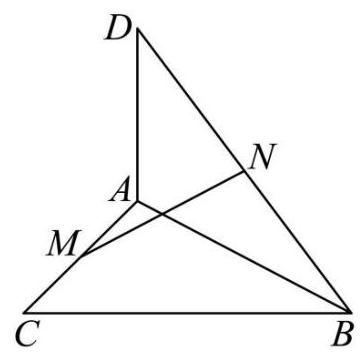
\includegraphics[max width=0.5\textwidth]{bo_d7ffh8ilb0pc73deo6o0_6_1131_1796_363_357_0.jpg}
\end{center}

(1)求证: \({MN}\bot {AC}\) ；

(2)若 \({AC} = {BC} = {AD} = 2\) ，求直线 \({MN}\) 与平面 \({ABD}\) 所成角的大小.
\end{questionblock}

\boardspace{1.5cm}

\begin{questionblock}{19}
某款足球机器人射点球时，射门点与球门中心的水平偏差(单位:cm)服从正态分布. 在正常状态下,偏差 \(X \sim  N\left( {0,{20}^{2}}\right)\) ,规定 \(\left| X\right|  > {60}\) 为“严重失误”.

(1)求一次射门出现严重失误的概率 \(p\) (精确到 0.0001)；

(2)假设每次射门相互独立，每次测试让机器人射门 16 次，若至少出现一次严重失误，则判定需要校准. 在正常状态下，求一次测试被判定需要校准的概率 \(\alpha\) (精确到 0.01 )，并说明该判定规则是否合理；

(3)因机械磨损，机器人射门精度下降，一次射门出现严重失误的概率增加到 5%. 此时每次测试仍射门 16 次, 但判定规则改为: 若至少出现 2 次严重失误, 才需要校准. 在磨损状态下, 求被判定需要校准的概率 \(\beta\) (精确到 0.01 ). 此时,若一次校准的成本为 1 万元,且每天测试 3 次,求日均校准成本的期望值 (精确到百元).

参考公式与数据:

①若 \(X \sim  N\left( {\mu ,{\sigma }^{2}}\right)\) ,则 \(Z = \frac{X - \mu }{\sigma } \sim  N\left( {0,1}\right)\) .

②若 \(Z \sim  N\left( {0,1}\right)\) ,则 \(P\left( {Z > 3}\right)  \approx  {0.00135}\) , \(P\left( {Z > 2}\right)  \approx  {0.0228}\) .

参考数据: \(\ln \left( {0.9973}\right)  \approx   - {0.002704},\;{0.95}^{16} \approx  {0.440},{0.95}^{15} \approx  {0.463}\) .
\end{questionblock}

\largeboardspace

\newpage

\begin{questionblock}{20}
已知椭圆 \(\Gamma  : \frac{{x}^{2}}{{a}^{2}} + \frac{{y}^{2}}{4} = 1\left( {a > 2}\right)\) 与直线 \({l}_{1} : y = \frac{x}{2}\text{ 、 }{l}_{2} : y =  - \frac{x}{2}\) . 过椭圆上一点 \(P\) 作 \({l}_{1}\) 的平行线交 \({l}_{2}\) 于点 \(M\) , 作 \({l}_{2}\) 的平行线交 \({l}_{1}\) 于点 \(N\) .

\begin{center}
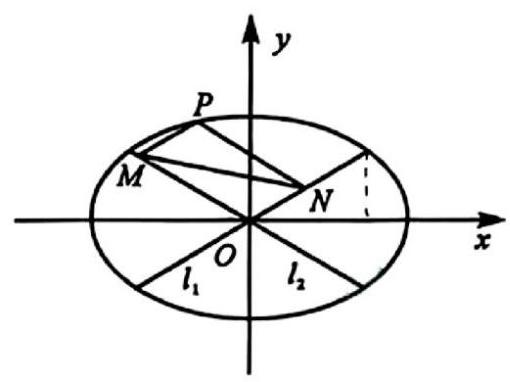
\includegraphics[max width=0.5\textwidth]{bo_d7ffh8ilb0pc73deo6o0_9_1013_591_510_382_0.jpg}
\end{center}

(1)当 \(P\) 为椭圆的上顶点时,求 \(\left| {MN}\right|\) 的大小;

( 2 )若椭圆的离心率 \(e = \frac{\sqrt{3}}{2}\) ，求椭圆 \(\Gamma\) 的方程，并求 \(\left| {\overrightarrow{OM} + \overrightarrow{ON}}\right|\) 的最大值与最小值;

(3)若 \(\left| {MN}\right|\) 为定值(与点 \(P\) 的位置无关)，求 \(a\) 的值，并求此时四边形 \({ONPM}\) 面积的最大值.
\end{questionblock}

\largeboardspace

\newpage

\begin{questionblock}{21}
已知在神经网络中, \(\sigma \left( x\right)  = \frac{1}{1 + {\mathrm{e}}^{-x}}\) 常作为神经元激活函数.

(1)证明:对任意实数 \(x\) ，有 \(\sigma \left( {-x}\right)  + \sigma \left( x\right)  = 1\) ，并由此写出 \(y = \sigma \left( x\right)\) 图像的对称中心；

(2)设交叉熵损失函数 \({L}_{t}\left( \widehat{y}\right)  =  - \left\lbrack  {t\ln \widehat{y} + \left( {1 - t}\right) \ln \left( {1 - y}\right) }\right\rbrack\) ，用于衡量预测值 \(\widehat{y}\) 与真实标签 \(t\) 之间的差异，其中 \(t \in  \{ 0,1\}\) . 试确定 \(t\) 的值,使得 \(z = {L}_{t}\left( {\sigma \left( x\right) }\right)\) 在 \(\left( {-\infty , + \infty }\right)\) 上是减函数;

(3)在深度神经网络中，信号经过多层传播可抽象为一个迭代过程. 设数列 \(\left\{  {x}_{n}\right\}\) 满足 \({x}_{n + 1} = \sigma \left( {x}_{n}\right)\) ，其中 \(n\) 为正整数. 证明: 存在唯一实数 \(A \in  \left( {0,1}\right)\) ,使得 \(\sigma \left( A\right)  = A\) ,且对任意实数 \({X}_{1}\) 和任意正整数 \(n\) ,都有 \(\left| {{x}_{n + 2} - A}\right|  \leq  {\left( \frac{1}{4}\right) }^{n}.\)
\end{questionblock}

\largeboardspace

\vfill
\begin{center}
\textit{— 试卷结束 —}
\end{center}

\end{document}